\section{Background And Motivation}

%\subsection{360-degree Tile-based Streaming}

%%In order to mitigate dependence on high bandwidth, FOV-aware tile-based streaming scheme, based on Dynamic Adaptive Streaming over HTTP (DASH) \cite{MPEG-DASH}, is extensively studied in recent years. For most typical works~\cite{Viewport-adaptive}\cite{360ProbDASH}\cite{Adaptive_Streaming_Framework} \cite{Two-tier}\cite{Omnidirectional_Video_over_HTTP}\cite{Furion}, 360-degree videos are split into segments of equal length, such as 1s, and the server offers multiple bit-rate of representations for every segment. Furthermore, with the technology of motion-constraint tile sets (MCTS), every segment can be encoded into multiple tiles spatially, as depicted in Figure 1, each of which can be independently decoded, stored into a single file and sent to clients alone. So, the server offers representations that also differ spatially by having a Quality Emphasized Region (QER)~\cite{Viewport-adaptive}: a region of the video which is made up of tiles with higher bit-rate than the rest of tile of the remaining of the video. Clients periodically pre-fetch a representation for the next segment such that the bit-rate adapts to available bandwidth and QER best matches the expected viewport of users.
%Unfortunately, these state-of-the-art works~\cite{360ProbDASH} \cite{Adaptive_Streaming_Framework} \cite{Two-tier} \cite{Omnidirectional_Video_over_HTTP} \cite{Furion}, which focus on the delivery of 360-degree video and only solved the problem of FOV-aware bit-rate adaptation in application layer, failed to design a effective FOV-aware scheme to guide the transport protocol to counter limited bandwidth and time-varying problem in mobile scenarios. 
%For example, they still use HTTP, built on top of TCP, as their transmission protocol. which, however, coupling flow and congestion control, suffers from poor throughput and delay performance in wireless networks featured by high loss rate, is inappropriate for 360-degree video delivery.

% Unfortunately, they only strive to optimize FOV-aware bit-rate adaptation schemes in application layer and failed to consider a effective FOV-aware scheme to guide the transport protocol. Thus, they can not perform well over lossy links, even worse in mobile scenarios.  

%However, even combined with 360-degree tile-based streaming, due to the failure to consider FOV, 

%\subsection{The introduction of FEC}
%	 MultiPath Parallel Transmission, considering mobile devices, like smartphone, almost equipped with diffrent radio interfaces (eg.Wi-Fi and LTE), is considered to be a promising way to solve the problem of limited bandwidth over wireless links. IETF-MPTCP \cite{IETF-MPTCP} is proposed and suffers from the performance degradation subject to the bottleneck link. These works~\cite{MPLOT}\cite{FMTCP} \cite{HMTP}, due to the introduction of FEC and well designed data allocation algorithm, not only aggregate capacities across paths but counter wireless network's time-varying characteristic, mitigating the head-of-line blocking and packet out-of-order in multiple diverse network.



	Generally, VR headset has a 110 degree horizontal FOV and a 90 degree vertical FOV, and the fraction of videos of video which extracted and displayed on HMD anytime would be $\frac{{110^\circ }}{{360^\circ }} \times \frac{{90^\circ }}{{180^\circ }}{\rm{ = }}15{\rm{\% }}$. Obvious, the data of the FOV region, viewed by users, is more important than non-FOV region.
	From the perspective of application layer, the FOV-aware tile-based streaming schemes, based on Dynamic Adaptive Streaming over HTTP (DASH), suggests that, 360-degree videos are split and encoded into multiple tiles spatially, each of which can be independently decoded, stored into a single file. Furthermore, according to the distance from the expected viewpoint of users, 360 videos would be split into two or three regions spatially, each of which would be composed of multiple contiguous tiles and store into a single file, as depicted in Figure 3.
	
	\begin{figure}[ht]
		\centering
		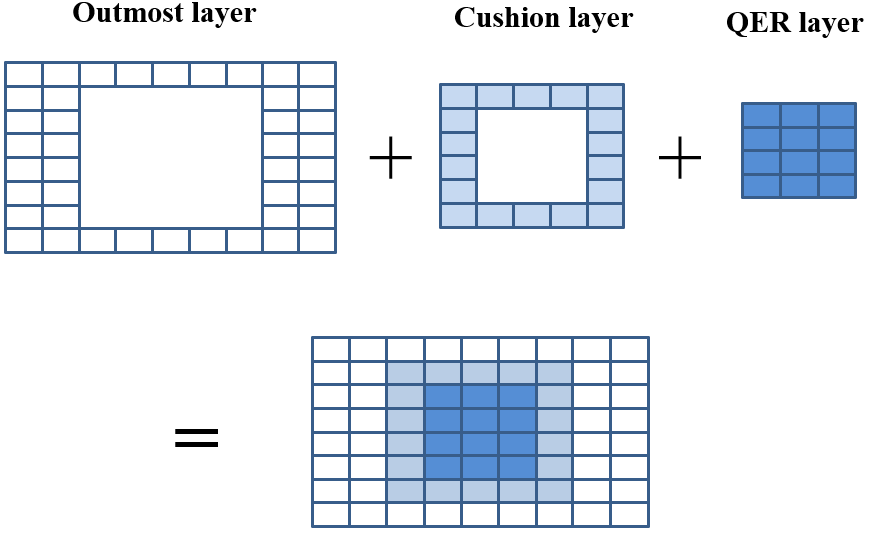
\includegraphics[scale=0.2]{paper_figs/tileSplit.png}
		\caption{360-degree Video Representation}
		\label{paper_figs:pathdemo}
	\end{figure}	
	
	
	However, the state-of-the-art transport schemes, which are not FOV-aware, spend as same amount of bandwidth on reliable delivery of trivial data, i.e., the non-FOV data, as the FOV data. So, can we, from the perspective of reliability of transport, design a protocol, which prioritizes the reliability of FOV data over non-FOV data, boosting the whole system performance by sacrificing little degree of quality of non-FOV data.

    
	Instead of only retransmissions, FEC\footnote{In Dante, FEC is generated through erasure coding of blocks of packets, to recover lost packets, which should be distinguished from FEC, computed on individual packets using channel coding, recovers from bit errors.} is adopted to be a proactive scheme of reliability in our proposed protocol. It can achieve low delay by mitigating retransmissions and is generally be in favoured by real-time video services. However, how to adjust the degree of FEC redundancy is a challenging problem. 
	 
	For example, considering a chunk of data organized into K packets, with equal length, the FEC encoder takes the K data packets, and adds M repair packets to create a coded block of size ${\rm{B = (K + M)}}$. The receiver can recover completely the origin data of K packets if any not less than K packets of all ${K + M}$ packets are received. The code rate is equal to ${K/(K + M)}$ and the redundancy of FEC is ${(M/K)}$ . Obviously, it can recover M packets of loss over lossy links at most and when FEC redundancy packets is more, the coding system has more powerful recoverability. 	 
	
    Increasing FEC redundancy can improve recovery probability of data packets in order to mitigate the degradation of video quality caused by packet transmission loss. However, with the increasing of redundancy and computing overhead of coding \cite{ASCOT}, the over-provisioning of redundancy may enlarge end-to-end delay, even causing unnecessary data loss caused by the hit of deadline. As depicted in Figure 2, with the increment of FEC redundancy, while the original data can be recovered with higher probabilities, the goodput first goes up to a peak point and degrades  latter, gradually. So, it's important to carefully adjust the redundancy of FEC in order to balance the tradeoff between recovery probability and goodput performance.  
	 
	We temporarily consider the situation where the video is split into two region, FOV region and non-FOV region. We find, instead of different regions encoded with the same FEC redundancy, it can lead to the better video quality that different regions are encoded with different FEC redundancy before the transmission. 
	 
    For example, the network status is set where average packet loss rate is set to 1\%, bandwidth is set to 40Mb/s. Meanwhile, the length of video segment is equal to o.5s, the size of FOV region is selected into 4Mb, the size of non-FOV region is 20Mb and playback deadline is set to 500ms. As illustrated in Table 1, while the set where all regions is encoded wih the same redundancy, perform worser among them the combination, the redundancy of FOV region and non-FOV is 2\% and 5\%, respectively, achieves obvious upgrade of video quality in FOV, and little degradation of video quality in non-FOV. Furthermore, FOV data, which is more likely perceived by users, is more important to QoE of video than non-FOV and the whole video quality is boost. So, when the network is limited-source and error-prone, if carefully designed, the schemes in which systems prioritized FOV data over non-FOV data, i.e., reliability VS best-effort, can effectively boost the whole system performance.       
	
	\begin{table}
		\centering 
		\scriptsize
		\begin{tabular}{p{2.0cm}p{2.0cm}p{1.6cm}p{1.6cm}}
			\rowcolor[gray]{0.9} 
			\hline
%			 The length of segment &The size of QER region(Mb) & The size of non-QER region(Mb) &
			The FOV redundancy(\%) &The non-FOV redundancy(\%) & Expected PSNR of FOV(dB) & Expected PSNR of non-FOV(dB)\\
			\hline
			3  &  3  &  35  &  35\\    
			\hline
			2  &  5  &  43  &  33\\ 
			\hline
			
		\end{tabular}
		\caption{The Video Quality of different FEC redundancy combinations}
		\label{}
	\end{table}
	 
	 
	Based on the above observations, unlike the 360-degree tile-based streaming schemes, which perform FOV-aware bit-rate adaptation on different region, we proposed Dante, the reliability scheme of which, performs on different region of videos in a hierarchical fashion, i.e, preferentially provisioning the data closer to FOV with more FEC redundancy. Thus, the data, which more strongly affects QoE of video, transmitted over lossy links, is supposed to integrally received with a higher probability and thus QoE of 360-degree video can be boosted notably.
 
%Manwhile, in Table 1, we summarize the main differences of Dante with the existing multipath schemes. 
To the best of our knowledge, Dante is the first FOV-aware 360-degree video protocol over heterogeneous wireless networks.
